
\begin{wrapfigure}{r}{3.5cm}
\centering
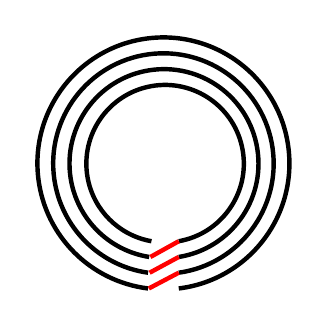
\begin{tikzpicture}[scale = 1]

\draw [ultra thick] (0,0) arc (-80:260:1);
\draw [ultra thick] (0,-0.2) arc (-81:261:1.2);
\draw [ultra thick] (0,-0.4) arc (-82:262:1.4);
\draw [ultra thick] (0,-0.6) arc (-83:263:1.6);

\draw [ultra thick, red] (0,0) -- (-0.36,-0.2);
\draw [ultra thick, red] (0,-0.2) -- (-0.37,-0.4);
\draw [ultra thick, red] (0,-0.4) -- (-0.38,-0.6);

\end{tikzpicture}
\caption{Domain representation with multiple windings}
\label{fig:winding_geom_scheme}
\end{wrapfigure} 

Magnets are usually made of a cable wound multiple times around the core. Creation of a CAD geometry where a cable is a single domain wound around the magnet bore $n$ number of times would be a complicated task. Therefore, in magnet analysis every winding  is considered as a separate domain, as shown in Fig. \ref{fig:winding_geom_scheme}. Then, the tips of the windings marked in red are coupled with the neighbouring ones thermally and electrically, i.e. they are characterised by the same temperature and voltage. With such an approach, one can easily create multi-dimensional magnet domains by specifying which windings are couple together. Moreover, with the same numerical domain, one can also analyse magnets wound in various manners depending on thermoelectric coupling applied to the winding tips. 

Multi-domain winding geometry allows for creation of a magnet geometry in 3D as well as for it thermoelectric analysis. Because of the multi-domain assumption, each winding may be characterised by one value of magnetic field and, therefore by one value of thermal and electrical material properties which depend on it. In quench velocity modelling, this 3D multi-domain geometry has to be mapped onto an imaginary 1D coil which is characterised by a length and number of windings~$n$. As presented in Fig. \ref{fig:ansys_python_mapping scheme}, each winding~$n$ can be characterised by a different value of magnetic field~$B_\text{n}$.

\begin{figure}[H]
\centering
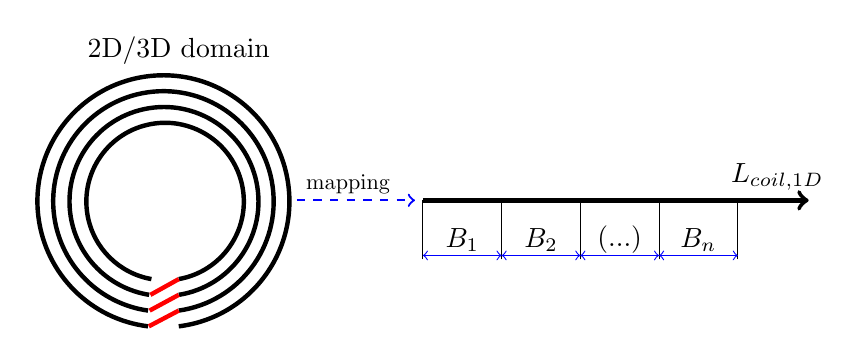
\begin{tikzpicture}[scale = 1]
\draw [ultra thick] (0,0) arc (-80:260:1);
\draw [ultra thick] (0,-0.2) arc (-81:261:1.2);
\draw [ultra thick] (0,-0.4) arc (-82:262:1.4);
\draw [ultra thick] (0,-0.6) arc (-83:263:1.6);
\draw [ultra thick, red] (0,0) -- (-0.36,-0.2);
\draw [ultra thick, red] (0,-0.2) -- (-0.37,-0.4);
\draw [ultra thick, red] (0,-0.4) -- (-0.38,-0.6);
\node[scale = 1.0] at (0,2.9) {2D/3D domain};
\draw [thick, dashed, blue, ->] (1.5,1) -- (3,1);
\node[scale = 0.8] at (2.15,1.2) {mapping};
\draw [ultra thick, ->] (3.1,1) -- (8,1);
\foreach \t in {3.1, 4.1, ..., 7.1}
\draw [thin] ({\t},0.25) -- ({\t},1);
\foreach \t in {3.1, 4.1, ..., 6.1}
\draw [thin, blue, <->] ({\t},0.3) -- ({\t+1},0.3);
\node[scale = 1.0] at (3.6,0.5) {$B_1$};
\node[scale = 1.0] at (4.6,0.5) {$B_2$};
\node[scale = 1.0] at (5.6,0.5) {(...)};
\node[scale = 1.0] at (6.6,0.5) {$B_\text{n}$};
\node[scale = 1.0] at (7.6,1.3) {$L_\text{coil, 1D}$};
\end{tikzpicture}
\caption{Multidimensional mapping scheme}
\label{fig:ansys_python_mapping scheme}
\end{figure}

Within the scope of numerical simulations presented in this thesis, it is assumed that the transverse heat propagation inside the windings is negligible with respect to the longitudinal one. Therefore, 1D elements are used to represent the winding domain. However, if a user wanted to represent the winding by means of 2D/3D elements in ANSYS, an extension has been made. Assuming that the nodes of each winding are placed in planes whose normal vector is aligned with the windings' direction, as shown in Fig. \ref{fig:ansys_python_mapping scheme_nodes}, the multi-dimensional domain can also be mapped onto the 1D imaginary Python cable. In such a case, the position of an imaginary Python node $N_\text{n}$ has the position which is an average position of all the nodes belonging to the plane $P_1$. 

It is worth mentioning that the set of nodes belonging to the first plane of one winding belongs to the same set of nodes as the last plane of the previous winding. This condition comes from the the fact that the tip nodes of the neighbouring windings should be coupled with one another. Therefore, the coupled nodes of different windings are considered in Python 1D imaginary coil geometry as the same node.

\begin{figure}[H]
\centering
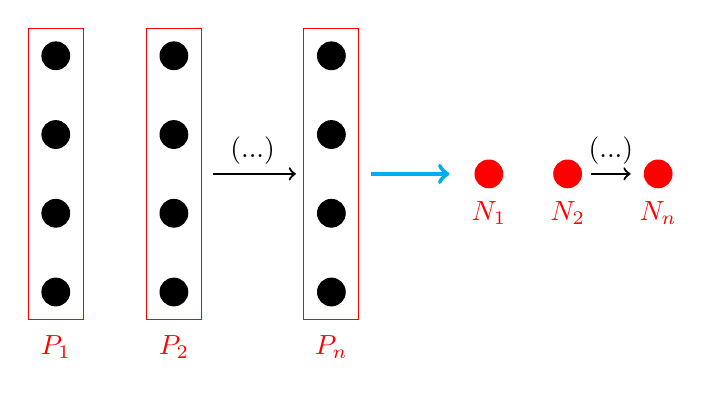
\begin{tikzpicture}[scale = 1]

\foreach \t in {0,1,...,3}
\filldraw[black] (0,{\t}) circle (5pt);
\foreach \t in {0,1,...,3}
\filldraw[black] (1.5,{\t}) circle (5pt);
\foreach \t in {0,1,...,3}
\filldraw[black] (3.5,{\t}) circle (5pt);
\draw[red] (-0.35,-0.35) rectangle (0.35,3.35);
\draw[red] (1.15,-0.35) rectangle (1.85,3.35);
\draw[red] (3.15,-0.35) rectangle (3.85,3.35);
\draw[thick,->] (2,1.5) -- (3.05,1.5);

\node at (2.5, 1.8) {(...)};
\node[red] at (0, -0.7) {$\text{P}_1$};
\node[red] at (1.5, -0.7) {$\text{P}_2$};
\node[red] at (3.5, -0.7) {$\text{P}_\text{n}$};

\draw[ultra thick,->, cyan] (4,1.5) -- (5,1.5);
\filldraw[red] (5.5,1.5) circle (5pt);
\filldraw[red] (6.5,1.5) circle (5pt);
\draw[thick,->] (6.8,1.5) -- (7.3,1.5);
\filldraw[red] (7.65,1.5) circle (5pt);

\node at (7.05, 1.8) {(...)};
\node[red] at (5.5, 1) {$\text{N}_1$};
\node[red] at (6.5, 1) {$\text{N}_2$};
\node[red] at (7.65, 1) {$\text{N}_\text{n}$};


\end{tikzpicture}
\caption{Plane assignment scheme}
    \label{fig:ansys_python_mapping scheme_nodes}
\end{figure}